\documentclass[12pt]{article}

% фонтови и језик
% fontspec docs: shorturl.at/ouI26
\usepackage{fontspec}

% polyglossia docs: shorturl.at/gELX9
\usepackage{polyglossia}
\newfontfamily\cyrillicfont{Times New Roman} % може се заменити компатибилним фонтом
\newfontfamily\cyrillicfontsf{Arial}         % може се заменити компатибилним фонтом
\newfontfamily\cyrillicfonttt{Courier New}   % може се заменити компатибилним фонтом
\setmainlanguage[Script=cyrillic]{serbian}
\setotherlanguage{english}

% вербатим линкови (веб адресе, имејлови, релативне адресе, итд.)
% url docs: shorturl.at/iktM4
\usepackage{url}

% хиперлинкови
% hyperref docs: shorturl.at/fmHPW
\usepackage{hyperref}

% приказивање математичких израза
% amsmath docs: shorturl.at/avJU3
\usepackage{amsmath}

% напредни пакет за исцрватање графика коришћењем команде \includegraphics
% graphicx docs: shorturl.at/diHUW
\usepackage{graphicx}
\graphicspath{{images/}}    % коренски директоријум слика, сваки пут када се користи includegraphics команда путања која се задаје треба да буде релативна у односу на овај директоријум

% рад са прилозима
% appendix docs: shorturl.at/uwEL1
\usepackage{appendix}

% подешавања маргина
\usepackage{vmargin}
\setmarginsrb{3 cm}{2.5 cm}{3 cm}{2.5 cm}{1 cm}{1.5 cm}{1 cm}{1.5 cm}

% исцртавање програмског кода
\usepackage{minted}

% подешавање размака линија текста
\usepackage{setspace}

% цртање табела
\usepackage{booktabs}

% додатни макрои за израду рада
\usepackage{rsvp}


\title{Паралелизација алгоритма за решавање судокуа}                         
\author{Александар Стојановић}                  
\newcommand{\studentindex}{E2 119/2023}    

\usepackage{fancyhdr}

\makeatletter
\let\thetitle\@title
\let\theauthor\@author
\let\thedate\@date
\let\theindex\studentindex
\makeatother

\pagestyle{fancy}
\fancyhf{}
\rhead{\theauthor}
\lhead{\thetitle}
\cfoot{\thepage}


\begin{document}
\begin{titlepage}
	\centering
    \vspace*{0.5 cm}
    
\includegraphics[scale = 0.75]{ftn-logo.eps}\\[1.0 cm]	                % University Logo
    \textsc{\LARGE Факултет техничких наука}\\[0.5 cm]	                    % University Name
	\textsc{\Large Универзитет у Новом Саду}\\[1.0 cm]				        % Course Code
	\textsc{\large Рачунарски системи високих перформанси}\\[0.5 cm]		% Course Name
	\rule{\linewidth}{0.2 mm} \\[0.4 cm]
	{ \huge \bfseries \thetitle}\\
	\rule{\linewidth}{0.2 mm} \\[1.5 cm]
	
	\begin{minipage}{0.4\textwidth}
		\begin{flushleft} \large
			\emph{Аутор:}\\
			\theauthor
			\end{flushleft}
			\end{minipage}~
			\begin{minipage}{0.4\textwidth}
			\begin{flushright} \large
			\emph{Индекс:} \\
			\theindex								                        % Your Student Number
		\end{flushright}
	\end{minipage}\\[2.0 cm]
	
	{\large \thedate}\\[2 cm]
	\vfill
\end{titlepage}

\pagenumbering{roman}              
%%%%%%%%%%%%%%%%%%%%%%%%%%%%%%%%%%%%%%%%%%%%%%%%%%%%%%%%%%%%%%%%%%%%%%%%%%%%%%%%%%%%%%%%%

% садржај
\tableofcontents
\pagebreak

%%%%%%%%%%%%%%%%%%%%%%%%%%%%%%%%%%%%%%%%%%%%%%%%%%%%%%%%%%%%%%%%%%%%%%%%%%%%%%%%%%%%%%%%%

% листинг изворних кодова
\listoflistings
\pagebreak

%%%%%%%%%%%%%%%%%%%%%%%%%%%%%%%%%%%%%%%%%%%%%%%%%%%%%%%%%%%%%%%%%%%%%%%%%%%%%%%%%%%%%%%%%

% листинг фигура
\listoffigures
\pagebreak

%%%%%%%%%%%%%%%%%%%%%%%%%%%%%%%%%%%%%%%%%%%%%%%%%%%%%%%%%%%%%%%%%%%%%%%%%%%%%%%%%%%%%%%%%

% листинг табела
%\listoftables
%\pagebreak

%%%%%%%%%%%%%%%%%%%%%%%%%%%%%%%%%%%%%%%%%%%%%%%%%%%%%%%%%%%%%%%%%%%%%%%%%%%%%%%%%%%%%%%%%

\pagenumbering{arabic}
\section{Увод}
Судоку је популарна загонетка са бројевима која се среће у многобројним дневним новинама  и часописима. Директан превод са јапанског имена ове загонетке је "јединствен број" што и осликава задатак ове игре, формирати квадратну матрицу димензија \(n \times n\) (најчешће 9х9) тако да се у свакој колони и врсти може затећи само једна појава бројева од 1 до \textit{n}. Исто правило примењује се и на одређене подматрице чије су димензије \(\sqrt{n} \times \sqrt{n}\). Играчу је на почетку игре дата матрица са неколико већ додељених вредности, а његов задатак је да матрицу попуни до краја, а да не прекрши правило јединствености појављивања бројева. Пример нерешене, а затим успешно решене загонетке може се видети на слици \ref{fig:unsolved_solved}.

\begin{figure}[H]
    \centering
    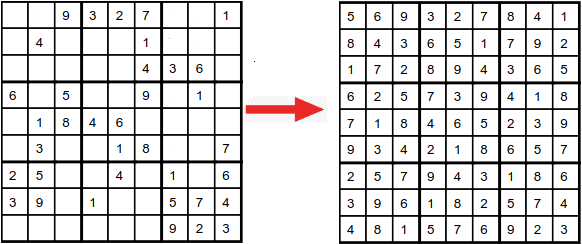
\includegraphics[width=1\textwidth]{images/unsolved_solved.png}
    \caption{Пример нерешеног и решеног судокуа}
    \label{fig:unsolved_solved}
\end{figure}

Циљ овог рада је паралелизација алгоритма за решавање ове загонетке. У даљим поглављима биће додатно појашњени основни појмови потребни за разумевање алгоритама, постојећа решења, а затим и ауторове имплементације овог алгоритма различитим приступима (\textit{openMP} примитиви и \textit{task}-ови, \textit{openMPI}), као и порeђење њихових перформанси.  
\pagebreak

\section{Основни појмови и постојећа решења}

Да би разумевање рада алгоритама за решавање ове загонекте било лакше, потребно је увести неколико основних појмова.\\

Појединачно поље у које се може сместити број назива се \textbf{ћелија}.\\

Ћелија која у датом тренутку решавања има само један број који је могуће уписати, без да се наруше ограничења, назива се \textbf{\textit{singleton}}.\\

Подматрица димензија \(\sqrt{n} \times \sqrt{n}\) која у себи мора садржати свих \textit{n} бројева назива се \textbf{\textit{box}}.\\

\textbf{\textit{Peer}}-ом се назива свака ћелија којa се налази у истој врсти, колони или \textit{box}-у (било која од ове три групације генерално се може називати \textbf{\textit{unit}}) у односу на посматрану ћелију.\\

Оно што је заједничко за све постојеће радове \cite{sudokuMulti,sudokuReport,sudokuMPI} као и ауторову имплементацију је то да се решавање загонетке заснива на два алгоритма, пропагацији ограничења и претрагом простора могућих решења.

\subsection{Пропагирање ограничења}
У уводном поглављу споменуто је основно ограничење загонетке које захтева да се унутар сваког \textit{unit}-а морају наћи сви бројеви и то тачно једном. Приликом решавања загонетке, ово ограничење се може рашчланити на два правила:
\begin{itemize}\label{rules}
    \item Ако се у некој од ћелија \textit{unit}-а посматране ћелије већ налази неки број, тај број се уклања из листе могућих бројева посматране  ћелије.
    \item Ако све ћелије \textit{unit}-a посматране ћелије сем ње имају одређен број избачен из њихове листе могућих бројева, тај број припада посматраној ћелији.
\end{itemize}

Узевши ова правила у обзир први корак решавања алгоритма била би њихова максимална примена широм целе матрице, све док се не дође до ситуације када још увек постоје празне ћелије, али немогуће их је попунити само на основу задатих правила.

\subsection{Претрага простора могућих решења}

Овај алгоритам полази од максимално попуњене матрице на основу правила из 2.1, затим користећи се скупом могућих бројева неке ћелије нагађа који би број могао стајати у њој и након тога наставља са пропагацијом ограничења, све док поново не дође до ситуације када мора да нагађа, ситуације када долази до крајњег решења или до контрадикторне ситуације. У случају проналаска решења алгоритам се овде завршава, а у случају контрадикторне ситуације алгоритам се враћа до последњег валидног стања матрице и покушава са новим бројем. Може се приметити да је овај алгоритам класичан пример \textit{back tracking} алгоритма \cite{backtrack}.\\  
\pagebreak

\section{Секвенцијална имплементација}\label{sec:sequential}
У овом поглављу биће описана секвенцијална имплементација, на којој ће се темељити и све наредне паралелне имплементације.

\subsection{Структуре података}

На почетку потребно је моделовати појединачну ћелију судоку матрице, као и читаву матрицу \ref{code:seq_structures}. Ћелија је прeдстављена као структура која од поља садржи коначну вредност (\textit{value}), која може варирати од 1 до \textit{n}, као и поље \textit{possibilities} којe ће се , ради уштеде меморијског простора, третирати као бинарни низ могућих вредности ћелије, где јединица на одређеном биту означава могућност појаве броја. На пример у случају 9х9 матрице број 0b1\_1010\_0010 значио би да су могуће вредности те ћелије бројеви 2, 6, 8 и 9. Читава матрица моделована је као дводимензионални низ ћелија. Уз ове структуре података имплементиране су и тривијалне помоћне методе за учитавање и писање матрице у \textit{csv} фајл, испис матрице на екран, копирање, као и проверу да ли је судоку решен тако што се проверава да ли све ћелије имају вредност у опсегу од 1 до \textit{n}, као и да им је низ могућих бројева једнак нули (0b0\_0000\_0000).

\begin{listing}[H]
\inputminted{c}{kodovi/seq_structures.c}
\caption{Неопходне структуре података}
\label{code:seq_structures}
\end{listing}

\subsection{Пропагирање ограничења}\label{constraint_prop}

Срж имплементације налази се у  \textit{solve} функцији, која се позива након учитавања нерешене судоку матрице. Као што је претходно поменуто, она се есенцијално састоји из два алгоритма, алгоритма за пропагирање   ограничења и алгоритма за претрагу простора могућих решења.\\

Пропагирање решења почиње применом претходно наведена 2 правила (\ref{rules}) над свим \textit{singleton}-има, а затим се у бесконачној петљи наизменично врше две акције. У првој се проналазе новонастали \textit{singleton}-и, додељује им се једини могући број и затим пропагирају ограничења која су произведена додавањем броја у ћелију. У другој акцији примењује се друго правило, где се за одређену ћелију проверава да ли постоји број који је избачен из низа потенцијалних бројева у свакоj од ћелија \textit{unit}-а посматране ћелије и ако је то случај ћелији се додељује тај број и пропагирају новонастала ограничења. Петља се прекида у тренутку када се нађе коначно решење (ово се може десити у лакшим загонеткама) или док се не примети да не постоји разлика у насталим судоку матрицама у претходне две итерације, што би значило да су ограничења максимално пропагирана и да је дошло време за претрагу простора могућих решења. Може се такође догодити ситуација када се пропагирањем ограничења дође у контрадикторно стање, у ком случају \textit{solve} функција враћа \textit{NULL} као решење. Овакво понашање битно је за наредни алгоритам.

\begin{listing}[H]
\inputminted{c}{kodovi/rules_propagation.c}
\caption{Пропагирање ограничења за ћелију}
\label{code:rules_propagation}
\end{listing}

\begin{listing}[H]
\inputminted{c}{kodovi/common_forbidden.c}
\caption{Имплементација примене другог правила}
\label{code:common_forbidden}
\end{listing}

Да се приметити да одлука за бинарну представу могућих бројева ћелије, поред уштеде меморијског простора, омогућава и ефикасније баратање низовима у овим случајевима коришћења где су итерације кроз низ у потпуности замењене бинарним операцијама О(1) комплeксности. У случају коришћења проналаска броја који је избачен из низа могућих бројева свих чланова \textit{unit}-а, сем из низа посматране ћелије \ref{code:common_forbidden} прво се свим низовима уради негација и тако добију сви забрањени бројеви, затим се комбиновањем свих низова помоћу бинарног "и" исфилитрирају бројеви и добију само они који су забрањени свим ћелијама. На крају се исфилтрирани низ забрањених бројева искомбинује са низом довољених бројева посматране ћелије, такође помоћу бинарног "и" и на тај начин добију бројеви који се могу уписати у ћелију. Ако се у низу налази само један број, он се одмах може уписати.

\subsection{Претрага простора могућих решења}

Након што се максимално испропагирају ограничења, прелази се на претрагу простора могућих решења \ref{code:seq_search}. Да нагађање не би било потпуно насумично, проналази се "оптимални кандидат" за нагађање, то јест ћелија која има најмањи број потенцијалних бројева. На овај начин минимизује се број гранања, а тиме и укупно време претраге у најгорем случају. Затим се пролази кроз сваки могући број посматране ћелије, додељује се ћелији и са тако измењеном судоку матрицом рекурзивно се позива \textit{solve} функција. Као што је поменуто у \ref{constraint_prop}, рекурзивна претрага наставља се све док се не дође до коначног решења или у случају доласка у контрадикторно стање матрице, где се онда алгоритам враћа до последњег валидног стања и даље покушава са другим бројем.

\begin{listing}[H]
\inputminted{c}{kodovi/seq_search.c}
\caption{Алгоритам претраге  простора могућих решења}
\label{code:seq_search}
\end{listing}  
\pagebreak

\section{Паралелна имплементација}\label{sec:parallel}

Анализом претходно описане секвенцијалне имплементације \ref{sec:sequential}, може се закључити да је готово немогуће паралелизовати део алгоритма који се бави пропагирањем ограничења, због тога што би свака промена ћелије захтевала синхорнизацију свих нити/процеса ради коректне даље пропагације ограничења, што би резултовало \textit{lockstep} паралелизацијом нити са великом фреквенцијом усклађивања. Са друге стране, алгоритам претраге простора могућих решења због свог  гранања на више независних претрага у дубину стабла могућих решења природно подлеже паралелизацији. Свака нит би модификовала судоку матрицу на другачији начин и тако започела своју претрагу за решењем и када би нека нит пронашла решење сигнализирала би крај претраге. На овај начин избегава се ситуација када би алгоритам узалудно претраживао велики део стабла због лоше почетне претпоставке \ref{fig:search_parallel}, a и свакако се убрзава сама претрага.

\begin{figure}[H]
    \centering
    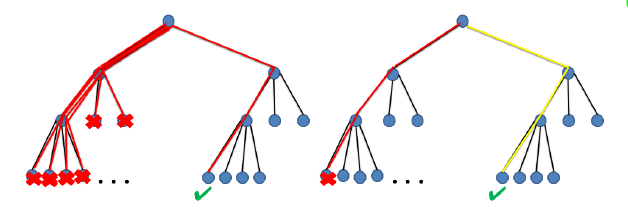
\includegraphics[width=1\textwidth]{images/search_parallel.png}
    \caption{Превенција узалудне претраге стабла уз помоћ паралелизације}
    \label{fig:search_parallel}
\end{figure}

\subsection{\textit{OpenMP} имплементација}\label{sec:mp_impl}

За разлику од постојећих решења која су се користила \textit{pthreads} \cite{pthreads} библиотеком, у овом пројекту је као алат за имплементацију изабран \textit{OpenMP} \cite{open_mp} ради декларативнијег приступа имплементацији.


\begin{listing}[H]
\inputminted{c}{kodovi/mp_search.c}
\caption{\textit{OpenMP} имплементација претраге}
\label{code:mp_search}
\end{listing}

За потребе паралелизације, петља унутар \textit{solve} функције која је служила за рекурзивну претрагу морала је подлећи одређеним модификацијама. Помоћу \textit{MP} директива, петља је паралелизована, тако да сада свака њена итерација која испробава један модел решења може да се извршава на засебној нити. Уместо да се резултат решења директно враћа из петље, сада се јавила потреба за дељеном променљивом \textit{finalResult} којој се приступа унутар критичне секције и уписује решење уколико се пронађе. Да би се одмах након проналаска решења прекинуо рад и свих осталих нити, уводи се још једна дељена променљива \textit{stopSignal}, чију вредност нит која је дошла до решења мења на \textit{true} и тако сигнализира свим осталим нитима да истог тренутка прекину са радом.

\subsection{\textit{OpenMP} имплементација употребом \textit{task}-ова}

Ова имплементација концептуално је слична \textit{MP} имплементацији преко примитива \ref{sec:mp_impl}. Разлика је у томе што сада само једна нит унутар петље креира \textit{task}-ове који се затим распоређују по свим нитима унутар паралелног региона \ref{code:mp_tasks_search}. Начин пропагације коначног решења и прекида рада свих осталих \textit{task}-ова остаје непромењен.

\begin{listing}[H]
\inputminted{c}{kodovi/mp_tasks_search.c}
\caption{\textit{OpenMP} имплементација претраге употребом \textit{task}-ова}
\label{code:mp_tasks_search}
\end{listing}

\subsection{\textit{OpenMPI} имплементација} 
Будући да се начин функционисања \textit{OpenMPI}-а \cite{open_mpi} разликује од \textit{OpenMP}-а, ова имплементација се знатно разликује од све три претходне.
Оно што разликује ову \textit{OpenMPI} имплементацију од постојећих је покушај делегирања посла једног процеса на све расположиве процесе, за разлику од тренутних имплементација где би процес био у могућности да половину свог посла делегира само суседном процесу (посматрајући \textit{id} процеса).\\

\subsubsection{Структуре података}

Поред постојећих структура података за ћелију и читаву судоку матрицу додат је низ \textit{unsigned} вредности \textit{availabilities} величине једнаке броју процеса који води рачуна о заузетости сваког од процеса. Такође било је потребно дефинисати нове \textit{MPI} типове података за размену ћелија и информација о доступности процеса између процеса \ref{code:mpi_structures}, као и написати помоћне функције за постављање судоку матрице у континуалан део меморије како би се она могла размењивати између процеса.

\begin{listing}[H]
\inputminted{c}{kodovi/mpi_structures.c}
\caption{Додатне структуре података}
\label{code:mpi_structures}
\end{listing}

\subsubsection{Хијерархија процеса и начин рада}

Читав рад заснива се на бесконачној петљи у којој се сви процеси налазе и чекају да им посао буде делегиран. Изузетак је процес са ранком 0, који је проглашен координатором који се бави вођењем евиденције о заузетости процеса и обавештавањем других процеса о тој информацији, као и очекивању коначног решења и финализацији алгоритма. Алгоритам почиње тако што координатор процес покушава пропагацију ограничења и ако из првог покушаја успе да реши загонетку одмах завршава програм, у супротном судоку матрицу са до тог тренутка максимално прорпагираним ограничењима прослеђује као задатак за решавање процесу 1 \ref{code:mpi_initial_cp}. 

\begin{listing}[H]
\inputminted{c}{kodovi/mpi_initial_cp.c}
\caption{Иницијална пропагација ограничења}
\label{code:mpi_initial_cp}
\end{listing}

Будући да би сви процеси требали да се баве својим задацима и асинхроно ослушкују да ли им је стигла нека порука, на разним местима у коду налази се слична конструкција која је приказана у коду \ref{code:mpi_message_waiting}. Сваки процес на почетку петље проверава да ли му је упућена нека порука и уколико јесте на основу њеног тага, одређује да ли се ради о поруци за завршетак процеса, поруци о прослеђеној матрици (решеној или спремној за обраду) или поруци за освежавање информације о доступности процеса.

\begin{listing}[H]
\inputminted{c}{kodovi/mpi_message_waiting.c}
\caption{Пример конструкције за  асинхроно ослушкивање порука}
\label{code:mpi_message_waiting}
\end{listing}

У код \textit{solve} методе коју позивају процеси када добију матрицу за обраду додато је неколико нових делова. На самом почетку ажурира се листа доступних процеса за делегирање посла и након пропагације ограничења пре него што се уђе у петљу за претрагу простора могућих ограничења процес прво делегира део посла свим доступним процесима\ref{code:mpi_job_delegation}. Након делегације посла, процес ће истражити преостале случајеве који нису делегирани. У случају проналаска решења оно се шаље директно координаторском процесу и завршава се програм.

\begin{listing}[H]
\inputminted{c}{kodovi/mpi_job_delegation.c}
\caption{Делегирање дела посла слободним процесима}
\label{code:mpi_job_delegation}
\end{listing}  
\pagebreak

\section{Поређење перформанси}
За мерење перформанси кориштени су примери судоку загонетки најтежег нивоа (\textit{evil}) и да би се додатно испровоцирао алгоритам за претрагу простора постојећих решења из тих примера обрисани су неки од бројева уз проверу да се њиховим брисањем није онемогућило решавање загонетке. Током тестирања мењан је број кориштених нити и процеса да би се уочио утицај паралелизације на брзину извршавања алгоритма. Модел процесора који је кориштен за тестирање је \textit{AMD Ryzen 7 7730U (base 2.0GHz, max 4.5GHz)}. Добијени су следећи резултати \ref{fig:seq_mp_results}\ref{fig:mpi_results}.

\begin{figure}[H]
    \centering
    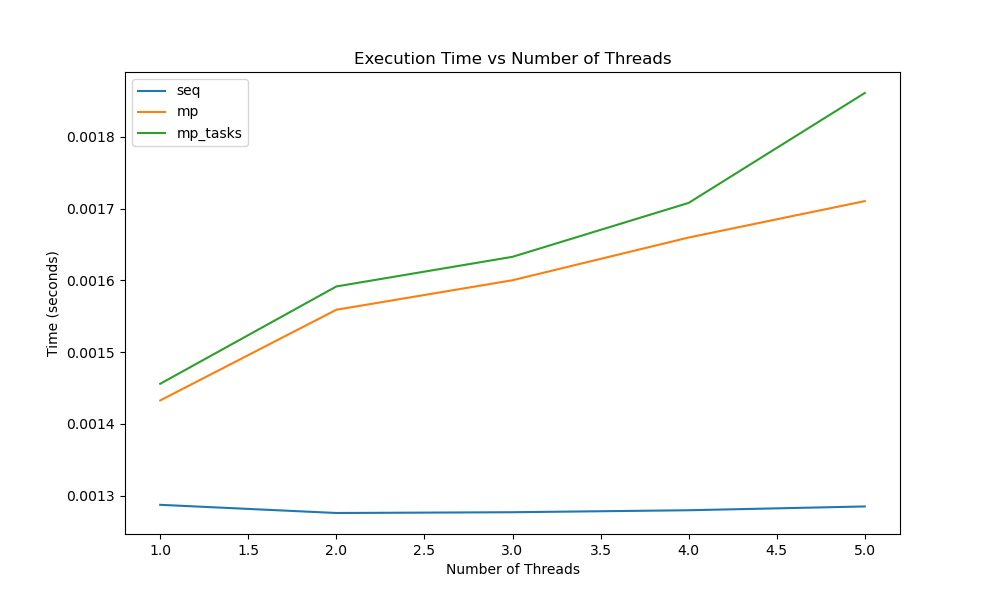
\includegraphics[width=1\textwidth]{images/graph_1.png}
    \caption{Резултати секвенцијалне и \textit{MP} имплементације}
    \label{fig:seq_mp_results}
\end{figure}

\begin{figure}[H]
    \centering
    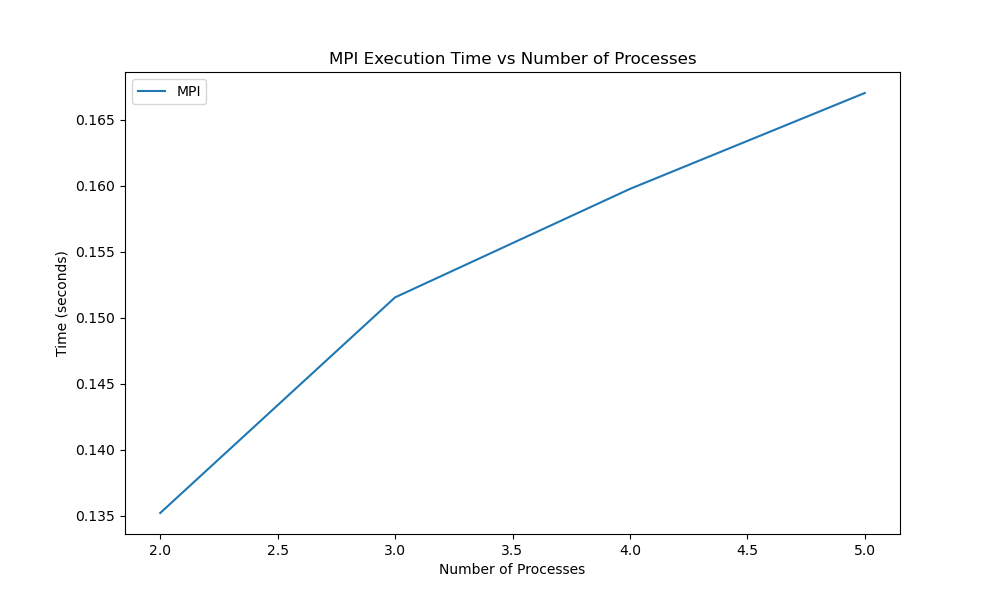
\includegraphics[width=1\textwidth]{images/graph_2.png}
    \caption{Резултати \textit{MPI} имплементације}
    \label{fig:mpi_results}
\end{figure}

На основу резултата да се уочити да је упркос разним покушајима паралелизације алгоритма за претрагу простора могућих решења, ипак секвенцијално решење најбрже и да се повећавањем броја нити и процеса само повећава \textit{overhead} потребан за координацију нити и процеса који додатно повећава време извршавања. Утицај на брзину секвенцијалног алгоритма највероватније има оптимизација алгоритма за пропагацију ограничења (проналажење оптималног кандидата и коришћење бинарног низа за складиштење могућих бројева), као и модернији модел процесора (мало мањи удео). Огромно одступање брзине \textit{MPI} имплементације оправдано је великим \textit{overhead}-ом који је потребан за координацију процеса, као и чинњеницом да се судоку матрица мора сваки пут трансформисати за потребе међусобне комуникације процеса, а њена величина није занемарљива.
  
\pagebreak

\section{Закључак}
У овом раду изучени су алгоритми који се користе за решавање судоку загонетке произвољне тежине (пропагација ограничења, претрага простора могућих решења), као и одређени приступи њиховој оптимизацији (бинарна представа могућих бројева ћелије, проналажење оптималног кандидата за даљу претрагу). Фокус је био на паралелизацији алгоритма за претрагу простора могућих решења. Проучаване имплементације користиле су се \textit{OpenMP} примитивима и \textit{task}-овима, као и \textit{OpenMPI}-ем и увеле неке нове приступе у односу на постојећа решења. Након мерења перформанси сваке од имплементацијa, дошло се до закључка да је секвенцијална имплементација ипак најбржа, због оптимизованости алгоритма за пропагирање ограничења и највећим делом \textit{overhead}-а који уводи потреба за координацијом нити и процеса. 
\pagebreak

\newpage
       
\newpage

\bibliographystyle{plain}
\typeout{}
\bibliography{biblist}             

\end{document}